%\documentclass[11pt,xcolor=gray,handout]{beamer}
\documentclass[hyperref={pdfpagelabels=false}]{beamer}
\let\Tiny=\tiny
\mode<presentation>{
\usetheme{Singapore}
%\usecolortheme{beaver}
\usefonttheme{serif}
}
\usepackage{default}
\usepackage{verbatim}
%\usepackage{ucs}
\usepackage[utf8]{inputenc}
\usepackage{gb4e}
\usepackage[T1]{fontenc}
\usepackage{ tipa }
\usepackage{qtree}
\usepackage{synttree}
\usepackage{color}
\usepackage{tree-dvips}
\usepackage[absolute,overlay]{textpos}
%\usepackage{covington-beamer}
\usepackage{lmodern}
\usepackage{natbib}
\usepackage{graphicx}
%\usepackage{pdfpages}


%\usepackage{memoir}
%\usepackage{relsize}
%\newcommand{\subscript}[1]{\raisebox{-0.25em}{\smaller #1}}
%\logo{\includegraphics[height=0.5cm]{hilogo2.png}}
\setbeamertemplate{footline}[frame number] 
%gets rid of navigation symbols
\setbeamertemplate{navigation symbols}{}

\title{Change, Stable Variation, and Why They're the Same Thing}
\author{Joel C. Wallenberg\\Newcastle University\\\texttt{joel.wallenberg@ncl.ac.uk}}
\institute{}
\date[]{December 17, 2013 \\ Seminaire de Récherche \\Université de Genève}

\begin{document}

\begin{frame}[plain]
\titlepage
\end{frame}


\section{Introduction}
\begin{frame}{Introduction}
	Variation in grammar is often described as falling into one of two categories.
	
	\begin{enumerate}
		\item Competing Grammars
		\begin{itemize}
			\item Leads to language change via the \textbf{replacement} of one grammatical process by another.
%			\item Competition is parameterized in some fashion, as in competing flavors of the same functional head \citep{kroch1994}.
		\end{itemize}
		\item Optionality (within a grammar?)
		\begin{itemize}
			\item Diachronically stable variation between grammatical processes.
		\end{itemize}
	\end{enumerate}
	
\end{frame}

\begin{frame}{Introduction}
	\textbf{Hypothesis:} all variation, including grammatical optionality, is formally \textbf{competing grammars}, with the following consequences \citep{fruehwaldwallenberg2013}:
	\begin{itemize}
		\item We expect variation (apparent optionality) between two grammatical forms to be diachronically unstable, generally.
		\item True optionality = stable variation, and its difference from language change must be explained by some mechanism of language use, outside of the grammar itself. 
%		\item The linguistic system (and therefore the variation) interacts with various dimensions of language use, which have their own characteristics. 
%the (in)stability of a competing grammars situation
		\item We argue that it depends on the mathematical character of some extragrammatical dimension (or external to the variable's grammar) with which the variation interacts.
			\begin{itemize} \item Partial specialization of variants along a continuous dimension. \end{itemize}
%		\item Optionality in grammar must also be parameterized. The implications of this point are greater for stable phonological variation.
	\end{itemize}

\end{frame}

\begin{frame}
\frametitle{Outline}
\tableofcontents
\end{frame}


\section{Blocking and Contrast}
%Maybe revise presentation
\subsection{How doublets resolve, and why.}
\begin{frame}
\frametitle{Blocking and Contrast}
\begin{block}{``Blocking Effect'' \citep{aronoff1976}}
	\begin{itemize}
		\item General cognitive pressure against two forms existing for one function (``doublet''), unstable \citep{kroch1994}.
		\item[ ]\{\textsl{lough, laughed}\} (laugh-\textsc{pst}; \citealt{taylor1994}) \\ \{\textsl{jimmies, sprinkles}\} (candy topping)
		%\item The possible historical outcomes of a doublet are replacement (one form left) or specialization (forms diverge in function).
	\end{itemize}
\end{block}
\begin{block}{``Principle of Contrast''}
	\begin{itemize}
		\item A strategy that children use in acquiring language: assume that two forms have two meanings (or uses)\citep[][{ \it inter alia}]{clark1987, clark1990}.
		\item Children hypothesize that novel words also refer to novel objects \citep[as in][among many other replications of the effect]{markmanwachtel1988}.
	\end{itemize}
\end{block}
%\begin{itemize}
%	\item General cognitive pressure against two forms existing for one function (``doublet''). 
%	\item This is the ``blocking effect'', as described for morphosyntactic doublets in Kroch (1994).\nocite{kroch1994}
%	\item The possible historical outcomes of a doublet are replacement (one form left) or specialization (forms diverge in function).
%	\item Crucially, they do not coexist forever, nor does one variant die randomly.
%	\item Part of the blocking effect is a language acquisition strategy, the ``Principle of Contrast'' (E. Clark 1987); \citep[cf. also][and references therein]{clark1990}. \nocite{clark1987}
%\end{itemize}
\end{frame}

\begin{frame}
\frametitle{The Principle of Contrast}
\begin{itemize}
	\item A strategy that children use in acquiring language: assume that two forms have two meanings (or uses) (E. Clark 1987, \textsl{inter alia}).
		\begin{itemize} \item Synonyms should only be acquired as a last resort.\end{itemize}
	\item Demonstrated in experiments such as \citet{markmanwachtel1988}.
		\begin{enumerate}
			\item 20 children
			\item 6 pairs of one familiar item (banana, cow, cup, plate, saw, spoon) and one unfamiliar item (cherry pitter, odd shaped wicker container, lemon wedgepress, radish rosette maker, studfinder, tongs).
			\item \textbf{Control}: ``Show me one''
			\item \textbf{Test}: ``Show me the X'' (X = nonsense syllable)
		\end{enumerate}
	\item Control children pick the unfamiliar object at chance levels, but test children choose unfamiliar objects significantly higher than chance.
\end{itemize}
\end{frame}


\begin{frame}
\frametitle{Blocking = Contrast + Selection}
\begin{itemize}
	\item A doublet is two variants competing for finite resources, as in e.g. biological evolution.
		\begin{itemize} 
			\item Instead of competing for something like food, they are competing for use (time in the mouths/brains of speakers). 
			\item \textbf{Selection} operates on the number of times a variant is heard (and accurately analyzed) by an acquirer.
			\end{itemize}
	\item Either one variant has an advantage, and so \textbf{replaces} the other \citep[following a logistic function;][]{nowak2006}.
	\item Or neither variant has an advantage (or much of one), in which case random walk and drift.
	\item But in linguistic doublets, random walk cannot persist indefinitely because of the acquisition pressure of the Principle of Contrast (\textbf{specialization}).
\end{itemize}
\end{frame}

\begin{frame}
\frametitle{Doublets = Competing Grammars \citep{kroch1994}}
\begin{itemize}
	\item[ ] \textbf{``Competing Grammars'', general form}: 2 variants are available to a speaker, in the relevant inventory of grammatical formatives, with overlapping functions (e.g. the same meaning).
		\begin{itemize}
			\item E.g. two featural versions of the same syntactic head. 
			\item E.g. two different output mappings for the same phonological input.
			\item E.g. two different Spell-outs of a morpheme.
		\end{itemize}
	\item[ ] A fact about language use: at some point in the derivation, the speaker reaches a \textbf{decision-point}.
		\begin{itemize}
		\item The speaker has a choice between formatives to continue the derivation, and either will result in a grammatical utterance and a meaning close enough to the speaker's intention.
		\item It is speaker ``choice'' more in the sense of an urn problem.
		\end{itemize}
		%SAY: the decision point exists because the different formatives exist, and that is competing grammars. Note that if they don't overlap in meaning, then the situation still exists formally, but there is no real decision 
		%Say something about adjunction
\end{itemize}
\end{frame}

\begin{frame}
\frametitle{Doublets = Competing Grammars}
\begin{itemize}
	\item Necessary for the description of \textbf{any} linguistic change in a categorical dimension.
		\begin{itemize} 
			\item E.g. word-order parameters \citep{pintzuk1991, santorini1992}; a phonological rule like German final stop devoicing (Fruehwald, Gress-Wright, \& Wallenberg 2009)\nocite{fruehwaldgresswallenberg}. 
			\item In any such case, a speaker in the middle of the change in progress (code-)switches between categorical variants \citep{kroch1989}.
		\end{itemize} 
\end{itemize}
\end{frame}


\begin{frame}{Summary: Blocking and Contrast}
	So, doublets are Competing Grammars, and the possible historical outcomes (\textbf{replacement}, \textbf{specialization}) are driven by selection and the Principle of Contrast.
%	\begin{itemize} 
%		\item Replacement of one by the other.
%		\item Specialization of the two forms to different functions or meaning.
%	\end{itemize}
\vspace{6mm}\\
	\textbf{Proposal:} every case of categorical linguistic variation or optionality can be reduced to Competing Grammars, leading to one of these two outcomes.
	\vspace{3mm}\\
	This simplifies the grammatical architecture necessary to account for both optionality and language change (in pursuit of a Minimalist hypothesis).
\end{frame}


%Talk more about Principle of Contrast

%
%\begin{frame}
%\frametitle{An Evolutionary Process}
%\begin{itemize}
%	\item Therefore, we propose that the Blocking Effect is reducible to Darwinian selection; it is just an evolutionary process.
%	\item A doublet resolves in replacement when one form has a selectional advantage.
%	\item A doublet resolves in specialization when neither form has a selectional advantage (or a very small one).
%	\item Unlike biology, the Principle of Contrast is built into acquisition and prevents random walk.
%	\item In biology, a selectional advantage is a higher probability of reproduction.
%	\item In language change, a selectional advantage is a higher probability of a child hearing and acquiring a particular structure.
%\end{itemize}
%\end{frame}
%
%
\section{Competing Grammars}

%
%\begin{frame}
%\frametitle{Polar Qs and Competing Grammars}
%\begin{itemize}
%	\item The competing grammars situation (like all morphosyntactic doublets) is constrained to two possible outcomes \citep{kroch1994}, as the \textsl{whether/if} study shows:
%		\begin{itemize}
%			\item Replacement of one variant by the other.
%			\item Specialization of each variant for a specific context over time.
%		\end{itemize}
%	\item \textbf{Proposal:} every case of syntactic variation or optionality can be reduced to competing grammars, in one of these two versions.
%	\item That is good, because competing syntactic heads is the only possible locus of variation/optionality in a BPS syntax.
%\end{itemize}
%\end{frame}
%
\subsection{Syntactic Optionality as Competing Grammars}
\begin{frame}
\frametitle{Example: English ``Topicalization''}
\begin{itemize}
	\item \citet{prince1985,prince1998, prince1999}: felicitous in two English discourse contexts, both of which require a certain type of contrast to appear on the fronted XP.
	
	\begin{exe}
\ex \label{princetop1} She's going to use three groups of mice.
One, she'll feed them mouse chow, just the regular stuff they make for
mice.
Another she'll feed them veggies.
And the third she'll feed junk food.\\

\ex \label{princetop2} She was here two years.
[checking transcript] Five semesters she was here.\\
\citep[][8,9]{prince1999} 

\end{exe}

	\item However, it is \textbf{never} obligatory.
\end{itemize}
\end{frame}
%
\begin{frame}
\frametitle{Example: English Topicalization}
\begin{itemize}
	\item As long as the accent pattern is kept constant, both orders are felicitous:
	
	\begin{exe}
\ex  She's going to use three groups of mice.
One, she'll feed them mouse chow, just the regular stuff they make for
mice.
Another she'll feed them veggies.
And \textbf{the third} she'll feed \textbf{junk food}.\\

\ex \label{untop1} She's going to use three groups of mice.
One, she'll feed them mouse chow, just the regular stuff they make for
mice.
Another she'll feed them veggies.
And she'll feed \textbf{the third} \textbf{junk food}.\\

\end{exe}

\end{itemize}
\end{frame}
%
%\begin{frame}
%\frametitle{Example: English ``Topicalization''}
%\begin{itemize}
%	\item As long as the accent pattern is kept constant, both orders are felicitous:
%	\begin{exe}
%
%\ex \label{princetop2} She was here two years.
%[checking transcript] \textbf{Five semesters} she was here.\\
%
%\ex \label{untop2} She was here two years.
%[checking transcript] she was here \textbf{five semesters}.\\
%
%\end{exe}
%
%\end{itemize}
%\end{frame}
%
\begin{frame}
\frametitle{Topicalization in Minimalism}
\begin{itemize}
	\item Move is triggered by the feature content of some head.
	\item Given ``Merge...preempts Move'' \citep{chomsky2000}, a feature cannot encode optional movement.
	\item Therefore, optional movement must involve a choice (for the \textbf{Numeration}) between two variants of a functional head, out of an inventory of possible heads:
\end{itemize}
\vspace{2mm}

\Tree [.CP XP_i [.C' {C\\$[F]$} \qroof{...t_i...}.TP ] ] \Tree [.CP C \qroof{...XP...}.TP ]

\begin{itemize}
	\item This is the core case of morphosyntactic doublet (i.e. competing heads) described in \citet{kroch1994}.
\end{itemize}

\end{frame}

\subsection{A Minimalist Hypothesis for Variation/Optionality}
\begin{frame}
\frametitle{A Minimalist Hypothesis}
\begin{itemize}
	\item[ ] Given that: 
		\begin{itemize} 
		\item these mechanics are necessary to encode syntactic optionality in a Minimalist system,
		\item the same mechanics are necessary to describe a change in progress,
		\end{itemize}
	\item[ ] Then, the system is simplest if no more machinery is added to deal with optionality/variation.
		\begin{itemize} \item Note: syntactic optionality represented as multiple formal (featural) versions of a functional head, competing for the speaker's choice in the speaker's inventory, is a logical consequence of the ``Borer-Chomsky Conjecture'' (\citealt{borer1984}, so named in \citealt{baker2008}).
		\end{itemize}
%SAY THE FOLLOWING OUT LOUD:
%	\item If the locus of variation between languages is a differing set of stored heads in the lexicon, then the locus of within speaker variation is also due to the set of stored heads in the lexicon, not something in the computational (combinatorial system).

\end{itemize}

\end{frame}

\begin{frame}
\frametitle{Minimalist Theory of Variation}
\begin{itemize}
	\item \textbf{Prediction:} every case of syntactic optionality or variation is one of the following:
		\begin{enumerate}
			\item A replacement change in progress (outright competition going to completion).
			\item A specialization change in progress (specialization for different functions going to completion).
			\item \textbf{``Stable'' variation, or optionality:} variants have partially specialized along a continuous (or ordinal) dimension, e.g. style, prosodic weight. 
		\end{enumerate}
	\item If categorical variants specialize along a categorical dimension, complete specialization should eventually result.
	\item If categorical variants specialize along a continuous or ordinal dimension, then complete specialization can \textbf{never} result, but replacement can still be ``arrested'' (\textbf{Caveat}).
\end{itemize}

\end{frame}

\subsection{Example: Embedded Polar Questions}

\begin{frame}
\frametitle{Example: Embedded Polar Questions}
A quantitative study of embedded \textsl{yes/no}-questions in English and Icelandic, comparing the use of \textsl{whether} vs. \textsl{if}, and \textsl{hvort} vs \textsl{ef} found \textbf{specialization} in English, and \textbf{replacement} in Icelandic (Bailey, Wallenberg, \& van der Wurff 2012). \nocite{baileywallenbergwurff2012}\\
	\begin{exe}
		\ex John wondered whether Mary was coming to the party.
		\ex John wondered if Mary was coming to the party.
	\end{exe}
\citet{baileywallenbergwurff2012} suggest the Proto-Gmc dual pronoun cognate with \textsl{whether} is reanalyzed as a polarity wh-word in clauses containing a disjunction.
\begin{center}
 \textbf{I asked \textsl{whether} (``which of two'') he wants, A or B.}% \\$\longrightarrow$ 
% \\ \textbf{I asked does he want A, or B?}
\end{center}
\end{frame}

\begin{frame}{Example: Embedded Polar Questions}
		In all stages of English and in historical Icelandic, a disjunction favors {\it whether}.
	\begin{block}{English}
		\begin{itemize}
		\item[ ]\textbf{Disjunction:}
		\begin{exe}
			\ex I wonder \{{\bf whether},if\} John or Bill is bringing coffee.
			\ex I wonder \{{\bf whether},if\} John is bringing tea or coffee.
			%\ex I wonder \{whether,if\} John is bringing tea or not.
		\end{exe}
		\item[ ]\textbf{Simple:}
		\begin{exe}
			\ex I wonder \{whether, {\bf if}\} Bill is bringing coffee.
		\end{exe}
		\end{itemize}
	
	\end{block}
\end{frame}

\begin{frame}{Example: Embedded Polar Questions}
%	\begin{block}{}
		\begin{itemize}
		\item[ ]\textbf{Disjunction:}
		\begin{exe}
			\ex \gll eftir því \textbf{hvort} maður vill heitt eða kalt\\
			according it-DAT whether man wants hot or cold\\
			\quad ``According to whether one wants hot or cold'' \\(\textsl{Sagan Öll}, date: 1985, from IcePaHC\nocite{icepahc09})
		\end{exe}
		\item[ ]\textbf{Simple, (older) Icelandic:}
		\begin{exe}
			\ex \gll vér vitum eigi, \textbf{hvort} vér tökum öndina\\
			We know not whether we take soul-the\\
			\ex \gll og spurðu, \textbf{ef} hann væri Kristur\\
			and asked if he were Christ\\
			(\textsl{Icelandic Homilies}, date: 1150, from IcePaHC)
		\end{exe}
		\end{itemize}		
%	\end{block}

\end{frame}

%\begin{frame}
%\frametitle{Persistence Effect}
%\begin{itemize}
%	\item This is a remarkably long-lasting ``persistence'' effect of the original reanalysis environment (cf. \textsl{have} vs, \textsl{have got} study by Shawn Noble, reported in \citealt{kroch1989}, cf. also \citealt{labov1989}).
%	\item Reanalysis: dual-meaning of \textsl{whether} to question-meaning of \textsl{whether}\citep{baileywallenbergwurff2012}.
%	\item[ ]\textbf{Disjunctive Yes/No Questions:}
%\begin{exe}
%	\ex I asked whether John wants tea or coffee.
%\end{exe}
%\end{itemize}
%\begin{center}
% \textbf{I asked which of the two he wants, A or B.} \\$\longrightarrow$ 
% \\ \textbf{I asked does he want A, or B?}
%\end{center}

%\end{frame}



%\begin{frame}
%\frametitle{A Quantitative Study}
%\begin{itemize}
%	\item A quantitative study of embedded \textsl{yes/no}-questions in English and Icelandic, comparing the use of \textsl{whether} vs. \textsl{if}, and \textsl{hvort} vs \textsl{ef}.
%	\item \textbf{Result 1:} A strong predictor of \textsl{whether} vs. \textsl{if} in both languages is the presence/absence of a disjunction (i.e. \textsl{or, eða}) in the clause, with \textsl{whether} being favoured in the disjunction case more than in the simple case in both languages, across their whole histories.
%	\item This indicates a remarkably long-lasting ``persistence'' effect of the original reanalysis environment (inspired by \textsl{have} vs, \textsl{have got} study by Shawn Noble, reported in \citealt{kroch1989}, cf. also \citealt{labov1989}).
%	\item The effect supports our hypothesis about the reanalysis environment.
%\end{itemize}
%\end{frame}


%\begin{frame}
%\frametitle{A Quantitative Study}
%\begin{itemize}
%	\item \textbf{Result 2:} The \textsl{whether} structure completely replaces the \textsl{if} structure in the Icelandic case, but not in the English case.
%	\item If the two possible outcomes of a morphosyntactic doublet are replacement or specialization \citep{kroch1994}, Icelandic shows the former and English shows the latter.
%	\item We propose that replacement must occur when there is some selectional advantage to one of the variants (in Darwinian terms, where reproduction = learning).
%	\item Specialization must occur when there is no selectional advantage to one of the variants.
%	\item \textbf{Experimental Infrastructure:} accurate parsed diachronic corpora: \small{ YCOE \citep{ycoe}, PPCME2 \citep{ppcme2}, PPCEME \citep{ppceme}, PPCMBE \citep{ppcmbe}, and IcePaHC \citep{icepahc09}.}
%	
%\end{itemize}
%\end{frame}
%
%\begin{frame}
%\frametitle{English Examples}
%\begin{itemize}
%\item[ ]\textbf{Disjunction:}
%\begin{exe}
%	\ex I wonder \{whether,if\} John or Bill is bringing coffee.
%	\ex I wonder \{whether,if\} John is bringing tea or coffee.
%	\ex I wonder \{whether,if\} John is bringing tea or not.
%\end{exe}
%\item[ ]\textbf{Simple:}
%\begin{exe}
%	\ex I wonder \{whether,if\} Bill is bringing coffee.
%\end{exe}
%\end{itemize}
%\end{frame}
%
%\begin{frame}
%\frametitle{Icelandic Examples}
%\begin{itemize}
%\item[ ]\textbf{Disjunction:}
%\begin{exe}
%	\ex \gll eftir því \textbf{hvort} maður vill heitt eða kalt\\
%	according it-DAT whether man wants hot or cold\\
%	\quad ``According to whether one wants hot or cold'' \\(\textsl{Sagan Öll}, date: 1985, from IcePaHC, \citealt{icepahc09})
%\end{exe}
%\item[ ]\textbf{Simple, (older) Icelandic:}
%\begin{exe}
%	\ex \gll vér vitum eigi, \textbf{hvort} vér tökum öndina\\
%	We know not whether we take soul-the\\
%	\ex \gll og spurðu, \textbf{ef} hann væri Kristur\\
%	and asked if he were Christ\\
%	(\textsl{Icelandic Homilies}, date: 1150, from IcePaHC)
%\end{exe}
%\end{itemize}
%\end{frame}
%
%\begin{frame} 
% \frametitle{English \textsl{whether} vs. \textsl{if} Questions, N = 1929 clauses}
%
%\begin{center}
% 
% \begin{textblock*}{125mm}(0mm,14mm)
%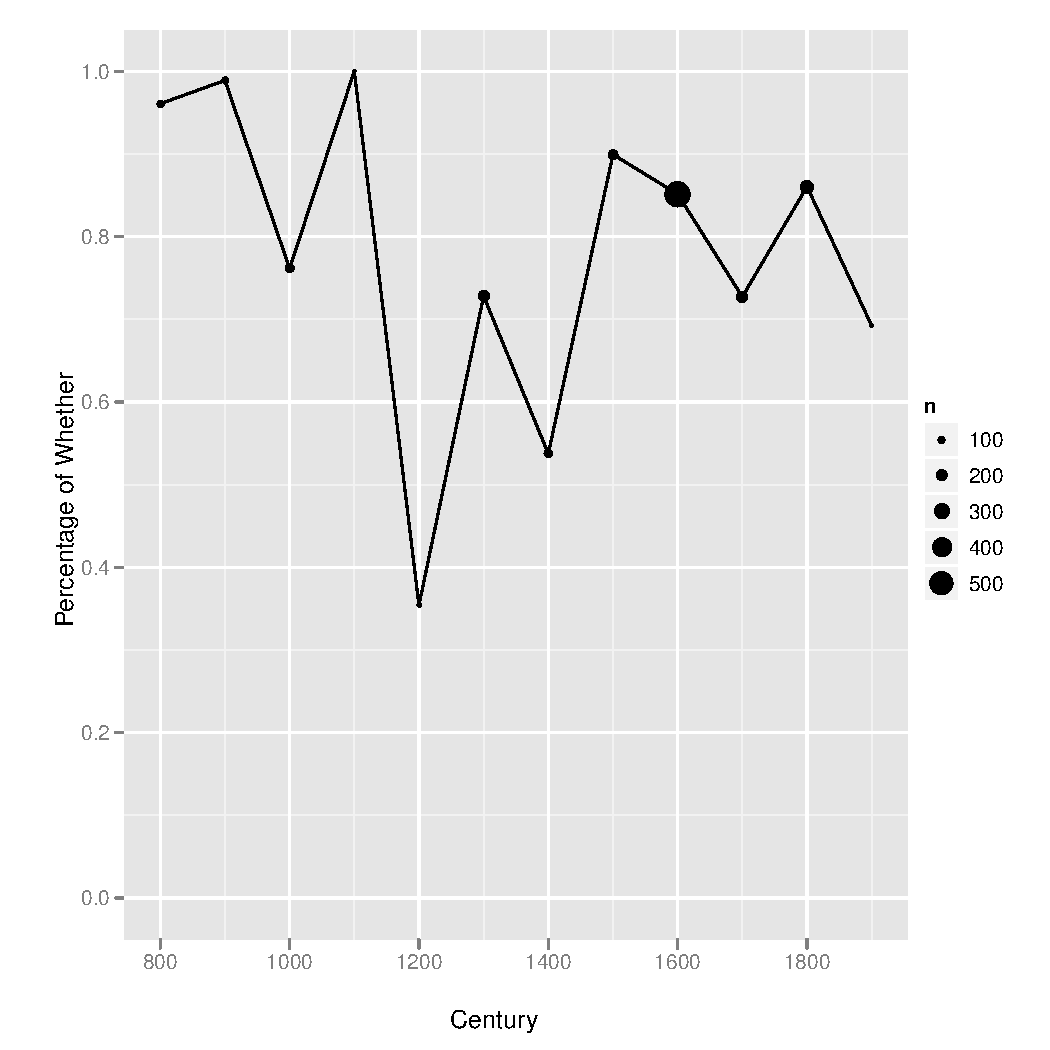
\includegraphics[width=109mm,height=82mm,clip=true,trim=0mm 0mm 0mm 0mm]{whetherifEngSimple.pdf}
%\end{textblock*}
%%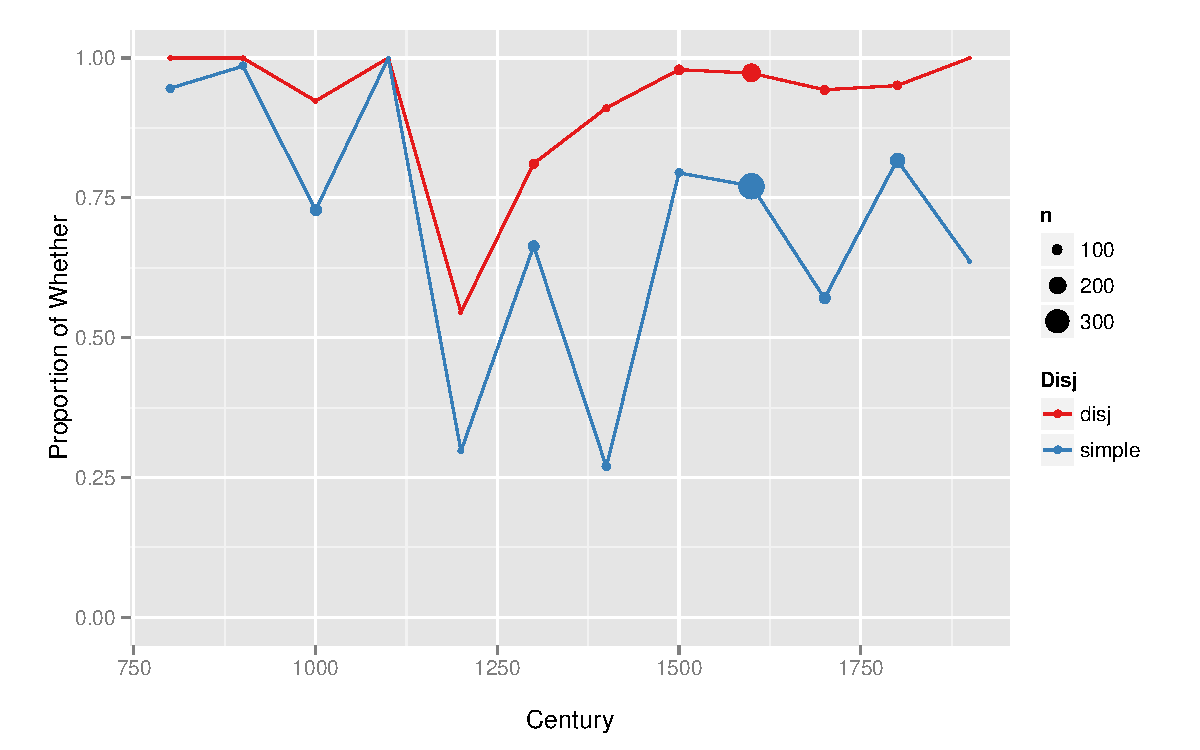
\includegraphics[scale = 0.5]{whetherifEng.pdf}
%\end{center}
%\end{frame}
%
%\begin{frame} 
% \frametitle{Icelandic \textsl{hvort} vs. \textsl{ef} Questions, N = 397 clauses}
%\begin{center}
% 
% \begin{textblock*}{125mm}(0mm,14mm)
%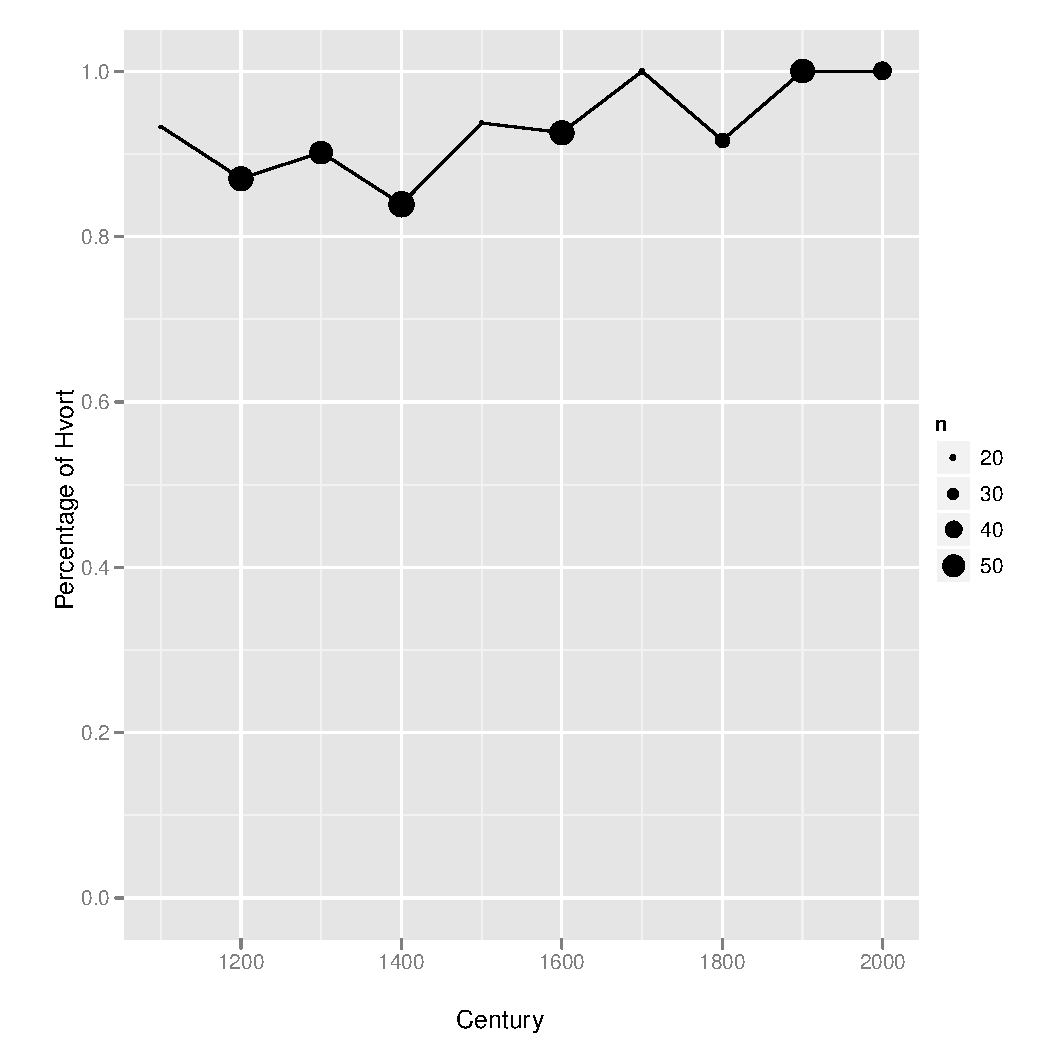
\includegraphics[width=109mm,height=80mm,clip=true,trim=0mm 0mm 0mm 0mm]{whetherifIceSimple.pdf}
%\end{textblock*}
%
%\end{center}
%\end{frame}
%
\begin{frame}{Specialization in English (N = 1929 clauses)} 


\begin{center}
 \small{Parsed Corpora: YCOE, PPCME2, PPCEME, PPCMBE \nocite{ycoe,ppcme2,ppceme,ppcmbe}}
% \begin{textblock*}{125mm}(0mm,14mm)
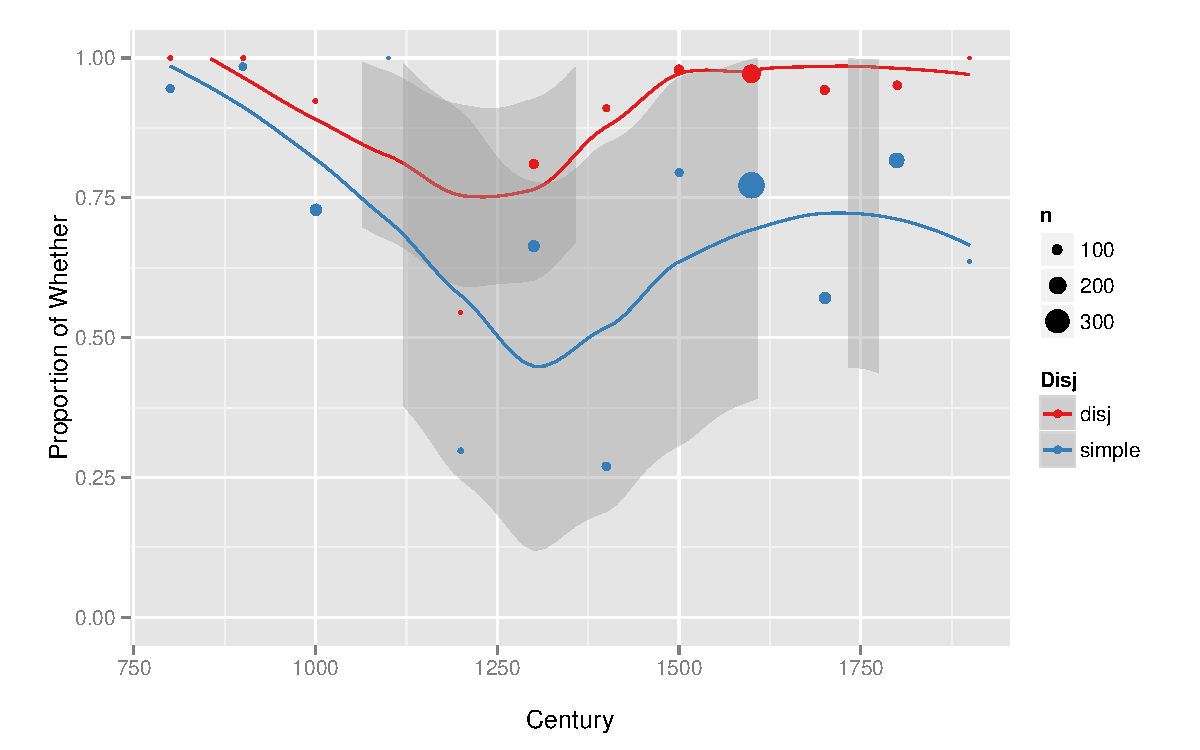
\includegraphics[width=1.1\textwidth]{whetherifEngLoess.pdf}
%\end{textblock*}
%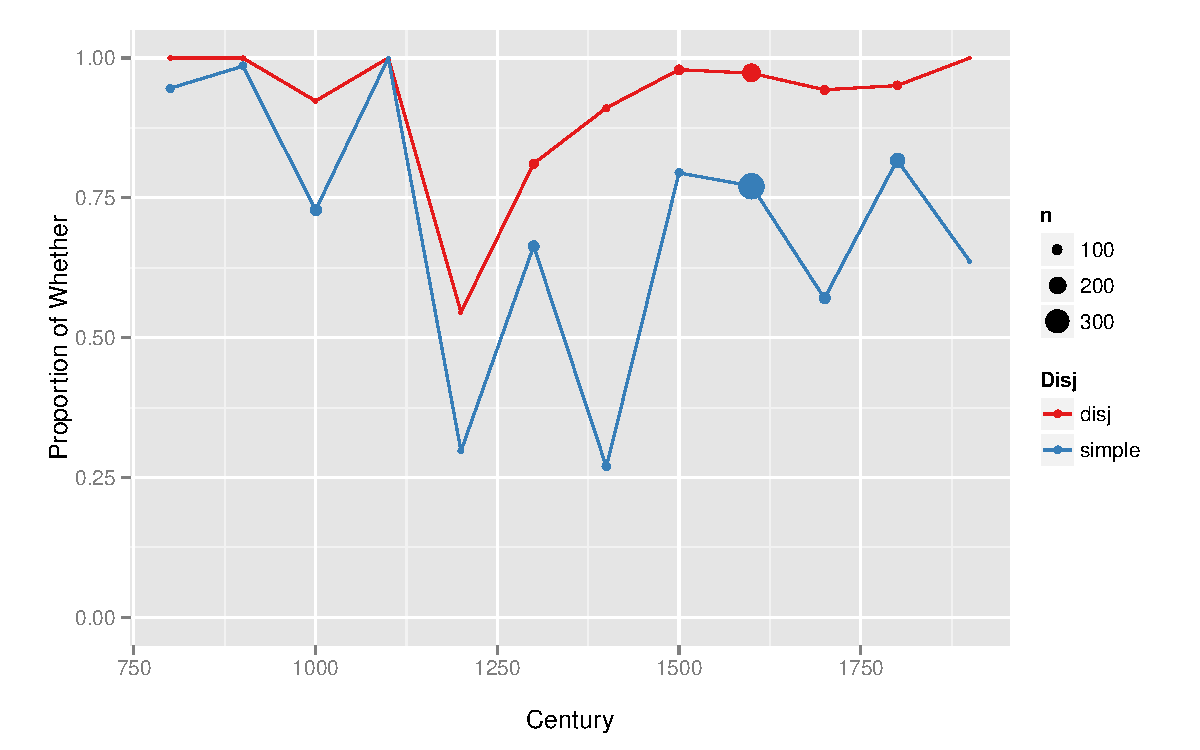
\includegraphics[scale = 0.5]{whetherifEng.pdf}
\end{center}
\end{frame}

%\begin{frame} 
% \frametitle{}
% \begin{center}
%                    
%\begin{tabular}{llllll}
%\hline
%  & Df & Deviance & Resid. Df & Resid. Dev &  Pr(>Chi) \\
%\hline
%NULL &   &    &            1928  &   1928.3 &  \\
%Disj   &    1 & 152.667  &    1927  &   1775.7 & < 2e-16\\
%Time     &    1  &  1.480  &    1926  &   1774.2  & 0.224\\
%Disj:Time  & 1  &  5.401   &   1925   &  1768.8 &    \textbf{0.0201}\\
%\hline
%\end{tabular}
%\end{center}
%\begin{itemize}
%\item A model without an interaction between Disjunction and Time fits significantly worse.
%\item Note that there is no clear effect of Time on \textsl{whether} use in general; the interesting effect is an interaction between Time, Disjunction, and  \textsl{whether} use.
%\item In other words, \textsl{whether} is not in decline, being replaced by \textsl{if}, but rather they are diverging from each other in use, specializing for the two contexts.
%\end{itemize}
%\end{frame}
%
%\begin{frame} 
% \frametitle{English, Logistic Model, N = 1929}
% \begin{center}
% \begin{textblock*}{125mm}(0mm,14mm)
%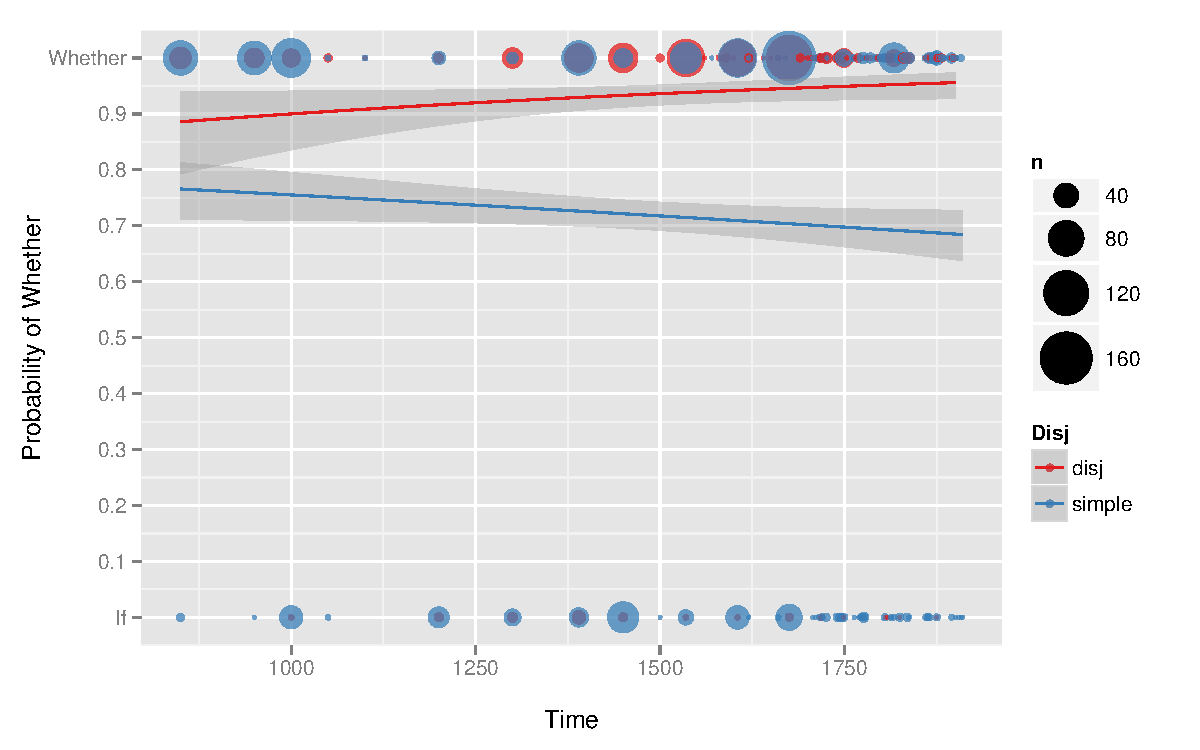
\includegraphics[width=109mm,height=80mm,clip=true,trim=0mm 0mm 0mm 0mm]{whetherifEngmodel.pdf}
%\end{textblock*}
% \end{center}
%\end{frame}
%
\begin{frame}{Replacement in Icelandic (N = 397 clauses)}

\begin{center}
IcePaHC \citep{icepahc09}
% \begin{textblock*}{125mm}(0mm,14mm)
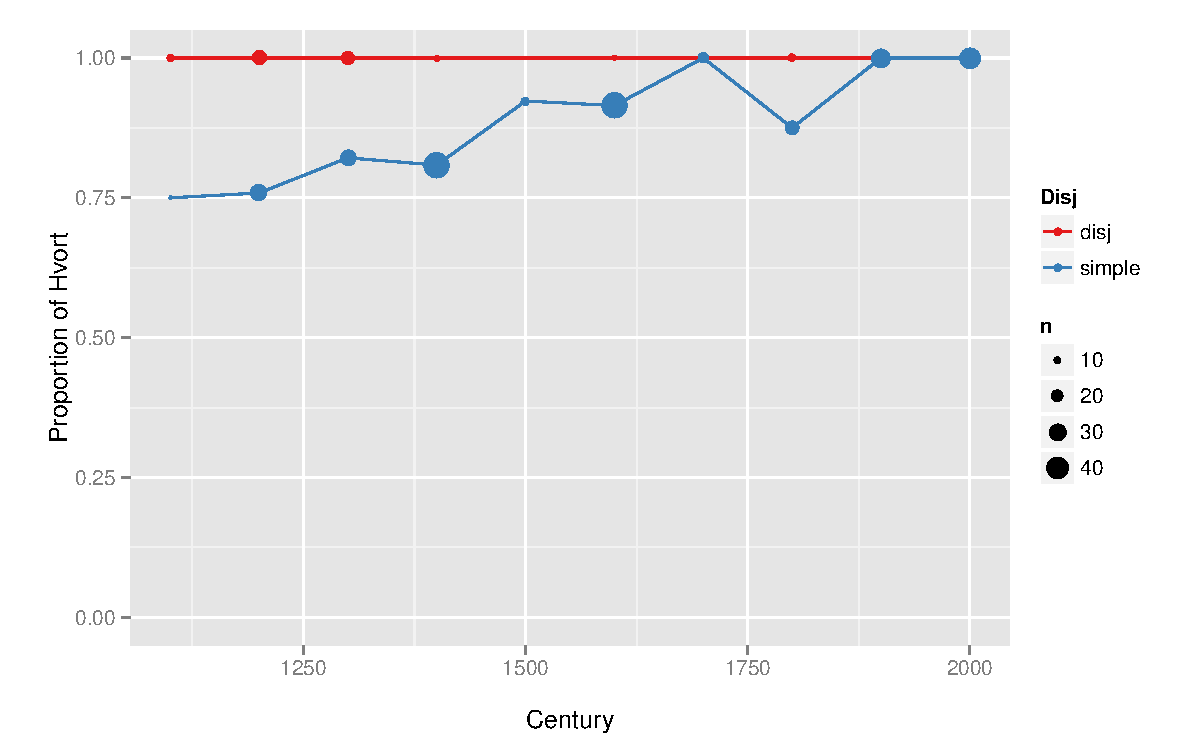
\includegraphics[width=1.1\textwidth]{whetherifIce.pdf}
%\end{textblock*}

\end{center}
\end{frame}

%\begin{frame} 
% \frametitle{Icelandic, Logistic Model, N = 397}
% \begin{center}
% \begin{textblock*}{125mm}(0mm,14mm)
%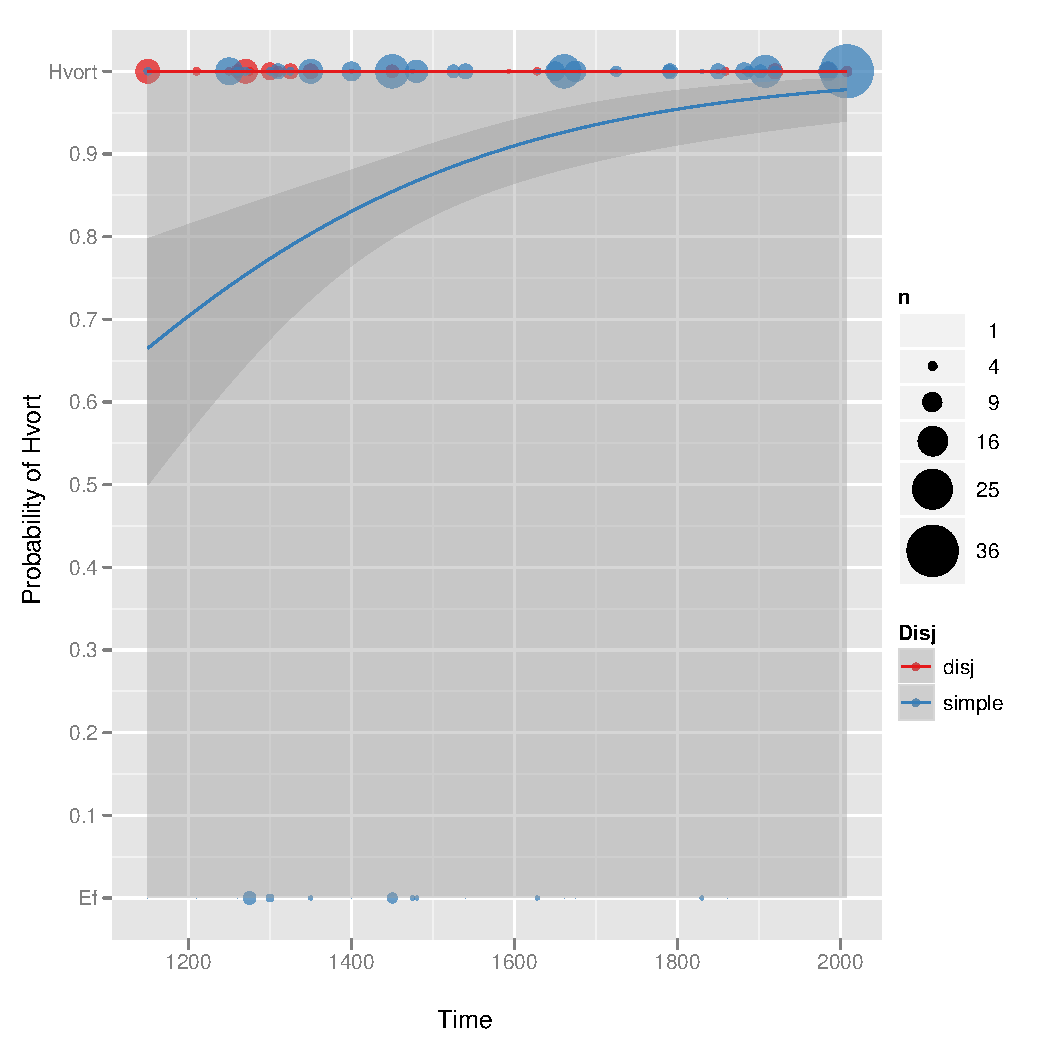
\includegraphics[width=109mm,height=80mm,clip=true,trim=0mm 0mm 0mm 0mm]{whetherifIcemodel.pdf}
%\end{textblock*}
% \end{center}
%\end{frame}
%
%
%\begin{frame}
%\frametitle{Whether/if Questions}
%
%\begin{exe}
%		\ex John wondered whether Mary was coming to the party.
%		\ex John wondered if Mary was coming to the party.
%\end{exe}
%\begin{itemize}
%	\item Is the frequency stable over time? Not in earlier English, but possibly in very recent history.	
%	\item Is it specialised for different speech styles (registers)? Yes, according to \citet{biberetal1999}.
%	\item Will they ever completely specialise for disjunction/simple? It depends on the strength of the style effect.
%\end{itemize}
%\end{frame}

%\section{Conclusions}
%\begin{frame}
%\frametitle{Conclusions}
%\begin{itemize}
%	\item We have shown that plausible reanalysis of \textsl{whether} in disjunctive contexts in Northwest Germanic led to its use in embedded \textsl{yes/no}-questions.
%	\item The effect of disjunctive contexts remains a crucial factor conditioning the choice between \textsl{if} and \textsl{whether} over the whole histories of English and Icelandic (in which it is categorical).
%	\item \textsl{whether} replaces \textsl{if} in Icelandic, but in English the two items specialise for different functions.
%	\item We suggested a reason for the difference between the two languages based on the continuing presence of the original reanalysis environment in Icelandic only (though this hypothesis would require more careful quantitative work to test).
%\end{itemize}
%\end{frame}
%
%\begin{frame}
%\frametitle{Conclusions and Future Research}
%\begin{itemize}
%	\item The data from the two languages illustrate the two possible outcomes for grammars that come into competition for use, according to the ``Blocking Effect''.
%	\item On the basis of this case study, we have suggested that the mechanism of competition for use could underlie all optional or variable syntactic phenomena, given:
%		\begin{itemize}
%			\item The Principle of Contrast as an acquisition strategy.
%			\item The mathematical nature of the dimension along which variants contrast (specialise).
%		\end{itemize}
%	\item Could we write a realistic, unified algorithm for acquisition, which predicts these effects? 
%\end{itemize}
%
%\end{frame}
%

\section{Stable Variation}
\begin{frame}
\frametitle{Stable Variation}
\textbf{Hypothesis:} Stable variation, i.e. optionality, results from categorical variants specializing along a continuous dimension.\\
\vspace{4mm}
There are many possible continuous dimensions, including language internal dimensions like
	\begin{itemize}
		\item weight (word or phrase length, or other prosodic measure)
		\item prosodic accent (number of aligned prosodic peaks, degree of stress clash between two positions)
	\end{itemize}
and language external dimensions like
	\begin{itemize}
		\item style
		\item speech rate
	\end{itemize}
\end{frame}

\subsection{Example: Topicalization}
\begin{frame}
\frametitle{Example: English Topicalization}

\begin{itemize}
	\item Is the frequency stable over time? Possibly since Late Middle English \citep{speyer2010}. (Though this is subject to revision).
	\item Is it specialized for different speech styles (registers)? Not that we know of.
	\item Is it sensitive to prosody? Definitely \citep{speyer2008, speyer2010}.
\end{itemize}
\end{frame}

\begin{frame}
\frametitle{Prosodic Sensitivity}
\begin{itemize}
%\item G. Ward's collection of modern English topicalizations shows that 90.5\% have pronominal subjects.
\item \citet{speyer2008, speyer2010} shows experimentally that prosodically ill-formed topicalization is subject to prosodic repair.
\end{itemize}
	\begin{exe}

	\ex  \textbf{The first group} she'll feed mouse chow, \textbf{the second} she'll feed veggies, and \textbf{the third} she'll feed  junk food.\\

	\ex  ? \textbf{The first} Caitlin will feed, \textbf{the second} Joe will feed, and \textbf{the third} Maggie will feed. \\

	\ex  ?? \textbf{Joel_i} Caitlin will pay \textsl{t_i}, \textbf{Bob_j} Joe will pay \textsl{t_j}, and \textbf{Ann_k} Maggie will pay \textsl{t_k}. \\
	
	\ex  ??? \textbf{Joel_i} Caitlin will pay \textsl{t_i} 10 dollars, \textbf{Bob_j} Joe will pay \textsl{t_j} 15 dollars, and \textbf{Ann_k} Maggie will pay \textsl{t_k} 20 dollars. \\

	\end{exe}
	
\end{frame}

\subsection{Example: -\textipa{In}$\sim$-\textipa{IN}}
\begin{frame}{Example: -\textipa{In}$\sim$-\textipa{IN}}
	\begin{exe}
			\ex John has been \{singing/singin'\}.
			\ex \{Dunking/Dunkin'\} Donuts.
	\end{exe}
	\begin{itemize}
		\item Is the frequency stable over time? Probably, as the variation has its roots in OE morphology (Houston 1985), and both variants were present in Middle English texts \citep{labov1989}.
		\item Is it specialized for different grammatical contexts? Yes, in part, along a nominal$\leftrightarrow$verbal dimension \citep{labov1989}.
		\item It it specialized for different speech styles? Yes, in part, along a continuous dimension of formality.
	\end{itemize}


\end{frame}

\subsection{Simulation: Acquisition of Specialization}
\begin{frame}{Example: -\textipa{In}$\sim$-\textipa{IN}}
	A proof of concept simulation shows that plausibly, under minimal acquisition assumptions:
	\begin{itemize}
	\item Variants specialize along a continuous dimension like style.
	\item For a continuous dimension, the process will stabilize at \textbf{partial} specialization (\textbf{Caveat}). 
	\item[ ] \begin{itemize}
		\item[\textbf{Gen 0:}]  -\textipa{In}$\sim$-\textipa{IN} doublet is innovated, with no stylistic conditioning. \textbf{Gen 0} picks a style to speak in, and produces a variant, repeats. 
		\item[\textbf{Gen 1:}]  \textbf{Gen 1} learns an estimate for the style value of -\textipa{In}, \textipa{IN}, as soon as she hears the first tokens of each from \textbf{Gen 0}. She adjusts this estimate as she gets more data from \textbf{Gen 0}.
		\item[\textbf{Gen 2:}] \textbf{Gen 1} picks a style, produces one of the variants with a probability weighted by how far her style estimates are from the current style, repeats. \textbf{Gen 2} learns style estimates for variants as above.
	\end{itemize}
	\end{itemize}
\end{frame}


%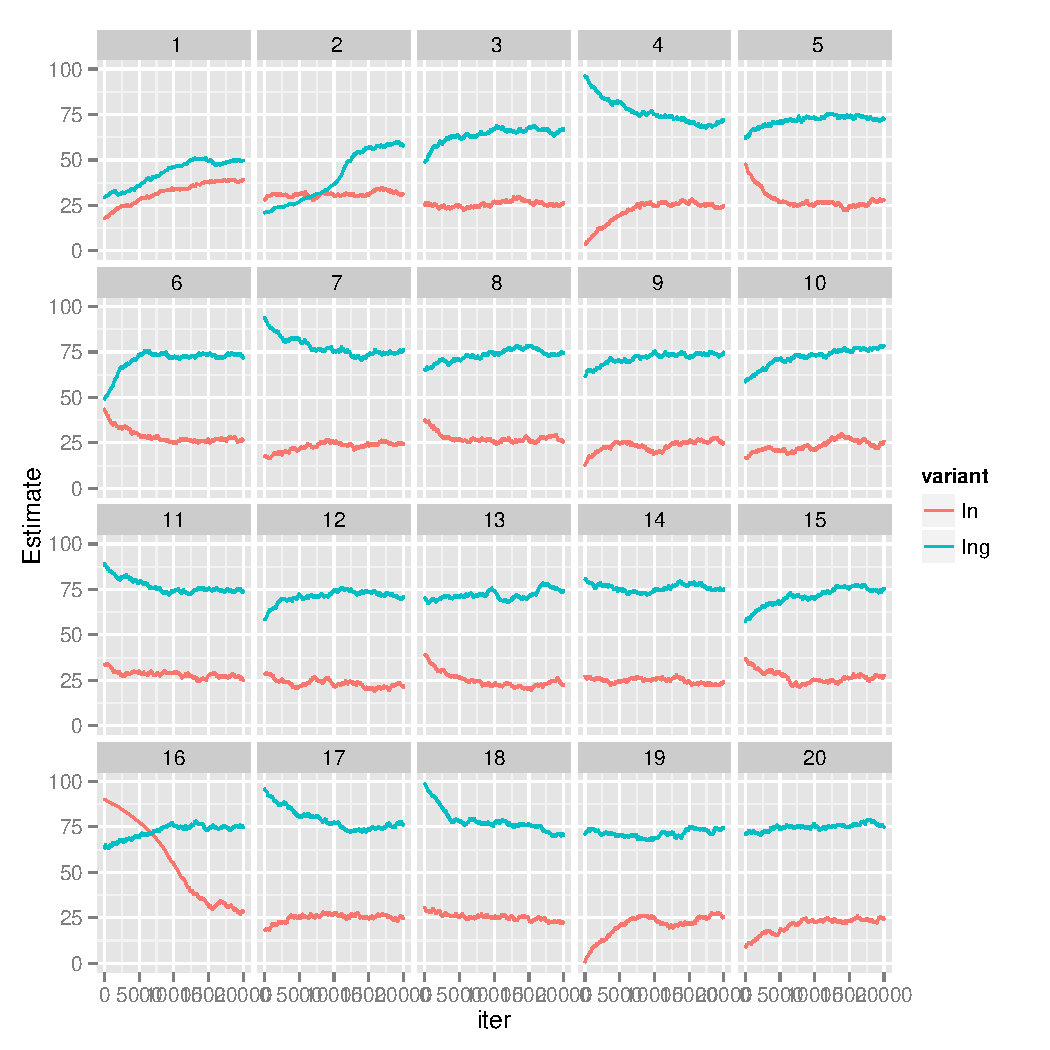
\includepdf{niceExample20000Run.pdf}

\begin{frame}{Instructive Observations from Simulation}
\begin{enumerate}
	\item We did not build the Principle of Contrast into the model. We just left the learner the possibility of contrasting the variants.
	\item There is no default style value for the variants. Their initial values are the first styles the learner hears from the last generation.
	\item The variants do specialize, but not all the way to the limits -- they stabilize at the quartiles (\textbf{Caveat}).
	\item Given 20000 tokens in each generation to learn from, the specialization stabilizes in about 4 generations.%of whether the variation results in specialization or replacement. (If the simulation is initialized by the first variants the adult utters -- this is important, because it is one *less* assumption in the model, i.e. there is no default value.)
\end{enumerate}
	\textbf{Open Question:} can we predict when specialization will occur successfully (or when replacement will happen instead)?
\end{frame}

\begin{frame}{When Specialization vs. Replacement?}
\begin{itemize}
	\item If neither variant has a selectional advantage, then specialization should occur (modulo \textbf{drift}).
	\item But if there is an advantage, then we have a race; who wins?
	\item First, the speaker must identify some \textbf{salient domain of specialization}.
	\item Specialization is driven by the Principle of Contrast, which is a fact about child cognition (i.e. should be as stable as the human brain).
\end{itemize}
\end{frame}

\begin{frame}{When Specialization vs. Replacement?}
\begin{itemize}
	\item Suppose, then, that specialization always occurs at the same rate per token of the linguistic variable that the child encounters.
	\begin{itemize}
		\item \textbf{Factor 1:} the size of selectional advantage for one variant vs. another, compared with the fixed rate of specialization.
		\item \textbf{Factor 2:} the frequency, in speech, of the context for the linguistic variable in question.
		\item Even if Factor 1 is small compared with rate of specialization, replacement could still occur if Factor 2 is small enough.
	\end{itemize}
	\item The specialization stabilizes at 20000 tokens, but with 1000 tokens it never does -- implies that the frequency of the variant could be a determining factor.
\end{itemize}
\end{frame}

%splice in 1000 run


%Talk to Joe about sound change in this perspective, how long it takes for speakers to id a domain of specialization for phonemic split

\subsection{Case Study: Relative Clause Extraposition}

\begin{frame}{Case Study: Relative Clause Extraposition}

	\begin{block}{French}
		\begin{exe}
			\ex \gll mais l'heure vient que je ne parleray plus a vous en proverbes\\
			but {the time} comes that I \sc{neg} speak-\sc{fut} more to you in proverbs\\
			\quad ``The time approaches when I will no longer speak to you in parables''\\
			(MCVF, 1523-NEW-TESTAMENT-P, A5V.2491)
		\end{exe}
	\end{block}
	
	\begin{block}{English}
		\begin{exe}
			\ex none lives that more loves you\\
			(PCEEC, TIXALL, 53.019.369, date: 1619)
		\end{exe}
	\end{block}

%\begin{block}{Icelandic}
%		\begin{exe}
%			\ex \gll stjarna væri sén í landnorðri frá Jemen, er Kómeta heitir\\
%			1861.ORRUSTA.NAR-FIC,.784)
%		\end{exe}
%	\end{block}

\end{frame}


\subsubsection{Within Speakers and Diachronically, PCEEC}

\begin{frame}{Within Speakers, and Diachronically}
\begin{itemize}
	\item Relative clause extraposition in the Parsed Corpus of Early English Correspondence  (PCEEC; \citealt{pceec}).
	\item Allows us to look at reasonable samples from individual speakers (letter-writers), as well as an historical sample from 1400--1700.
	\item Coded for prosodic weight of the relative clause, in number of words, from 0--50.
	\item Also coded for extraposition from Subject vs. Object.
\end{itemize}
	\textbf{Hypothesis:} individual speakers treat weight as a continuous variable, with extraposition specialized imperfectly along it, in roughly the way the acquisition model predicts \citep[following on][]{antonmackenzie2011a}.

\end{frame}


%Draw Normal plot

%Splice in two plots of speakers

\begin{frame}{All PCEEC, over time (N = 8073 clauses)}

\begin{center}
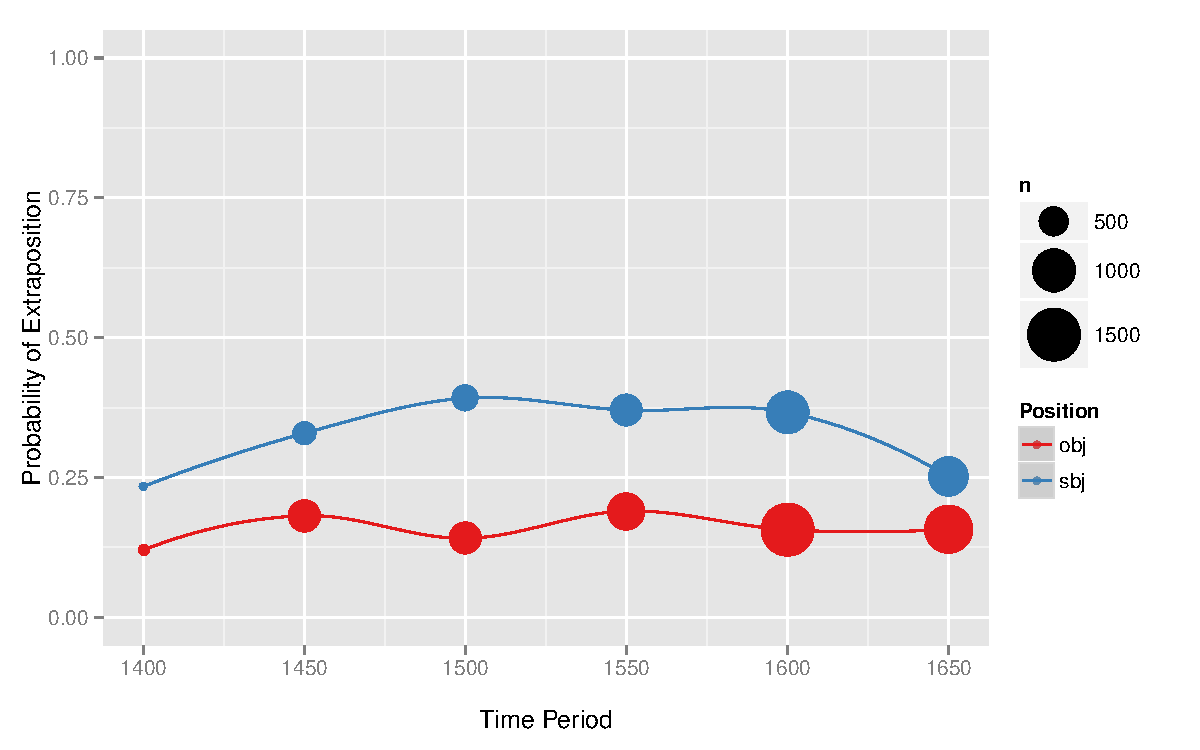
\includegraphics[width=1.1\textwidth]{exSbjObjYearBinned50.pdf}
\end{center}
\end{frame}


\subsubsection{Diachronically, Crosslinguistically}

\begin{frame}{Diachronically, Crosslinguistically}
\begin{itemize}
	\item \textbf{English:} YCOE \citep{ycoe}, PPCME2 \citep{ppcme2}, PPCEME \citep{ppceme}, PPCMBE \citep{ppcmbe}.
	\item \textbf{Icelandic:} IcePaHC \citep{icepahc09}.
	\item \textbf{Old/Middle French:} MCVF Corpus (Martineau, Hirschbühler, Kroch, \& Charles Morin, 2010) \nocite{mcvf}
	\item \textbf{Historical Portuguese:} Tycho Brahe Corpus of Historical Portuguese \citep{tychobrahe}.
	\end{itemize}
	\textbf{Hypothesis 1:} the specialization for weight has stabilized, so the effect of weight will be constant over time. \textbf{(Confirmed!)}
	\textbf{Hypothesis 2:} the overall rate of relative extraposition will be stable over time. \textbf{(Rejected!)}

\end{frame}

\begin{frame}{English, over time (N = 18530 clauses)}

\begin{center}
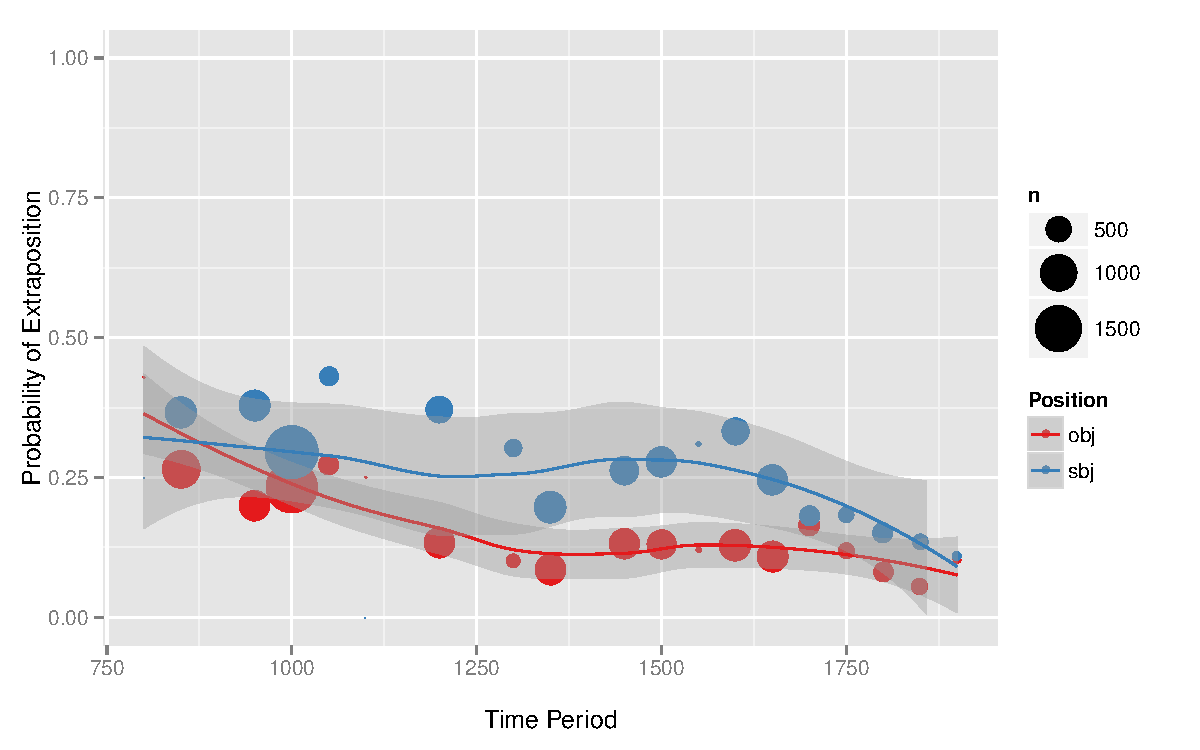
\includegraphics[width=1.1\textwidth]{exSbjObjYearBinned50Loessymeb.pdf}
\end{center}
\end{frame}

\begin{frame}{Not usual...cf. \citet{wallenberg2013}, N = 1030 clauses}

\begin{center}
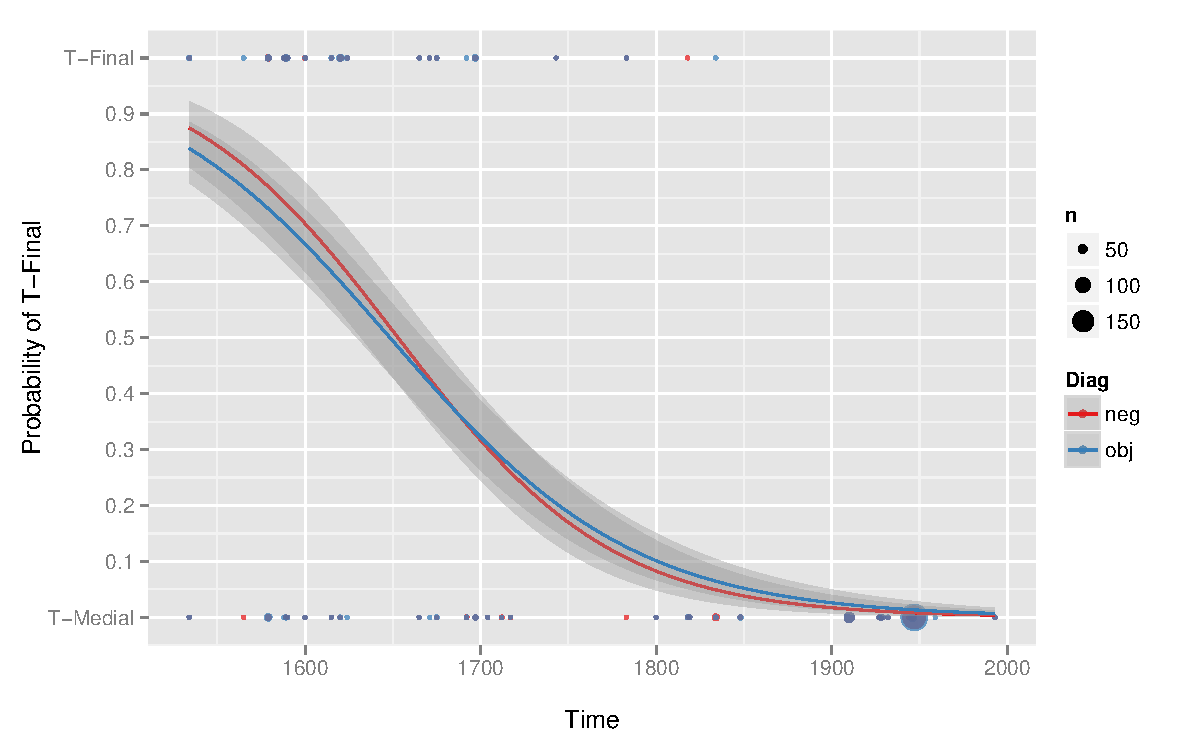
\includegraphics[width=1.1\textwidth]{yiddishLogistic.pdf}
\end{center}
\end{frame}


\begin{frame}{English, over time (N = 18530 clauses)}

\begin{center}
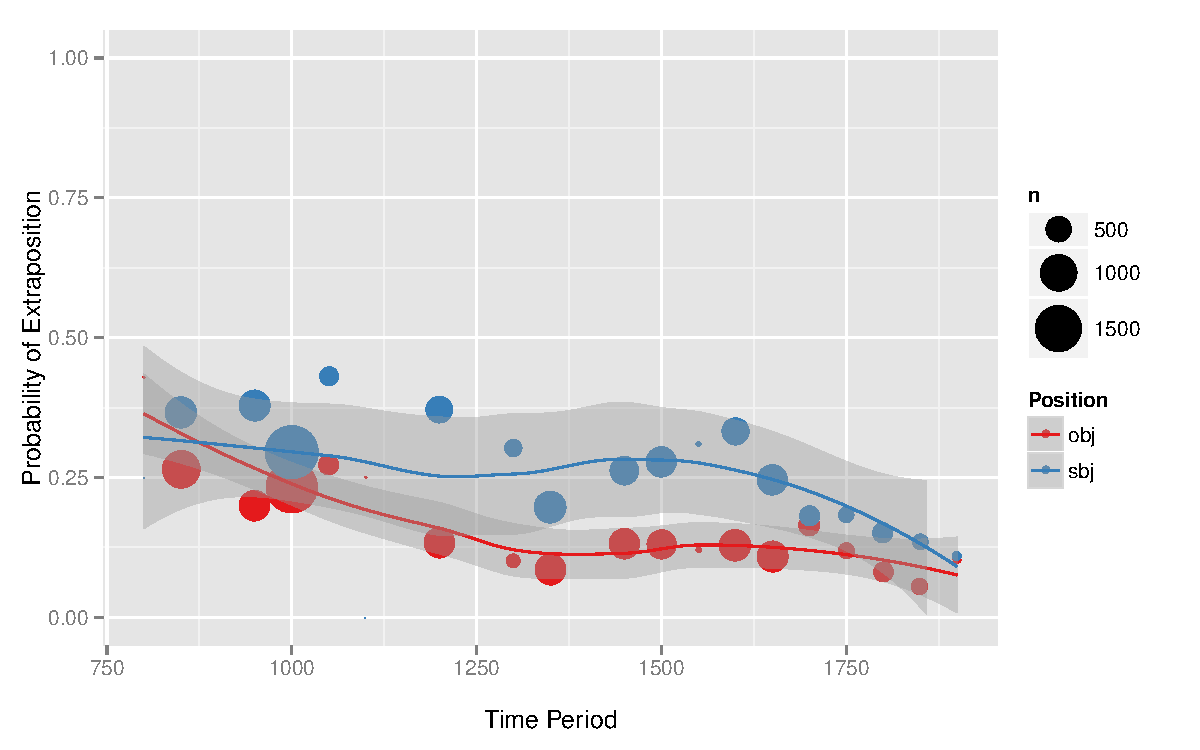
\includegraphics[width=1.1\textwidth]{exSbjObjYearBinned50Loessymeb.pdf}
\end{center}
\end{frame}


\begin{frame}{English, average weight over time (N = 18530)}

\begin{center}
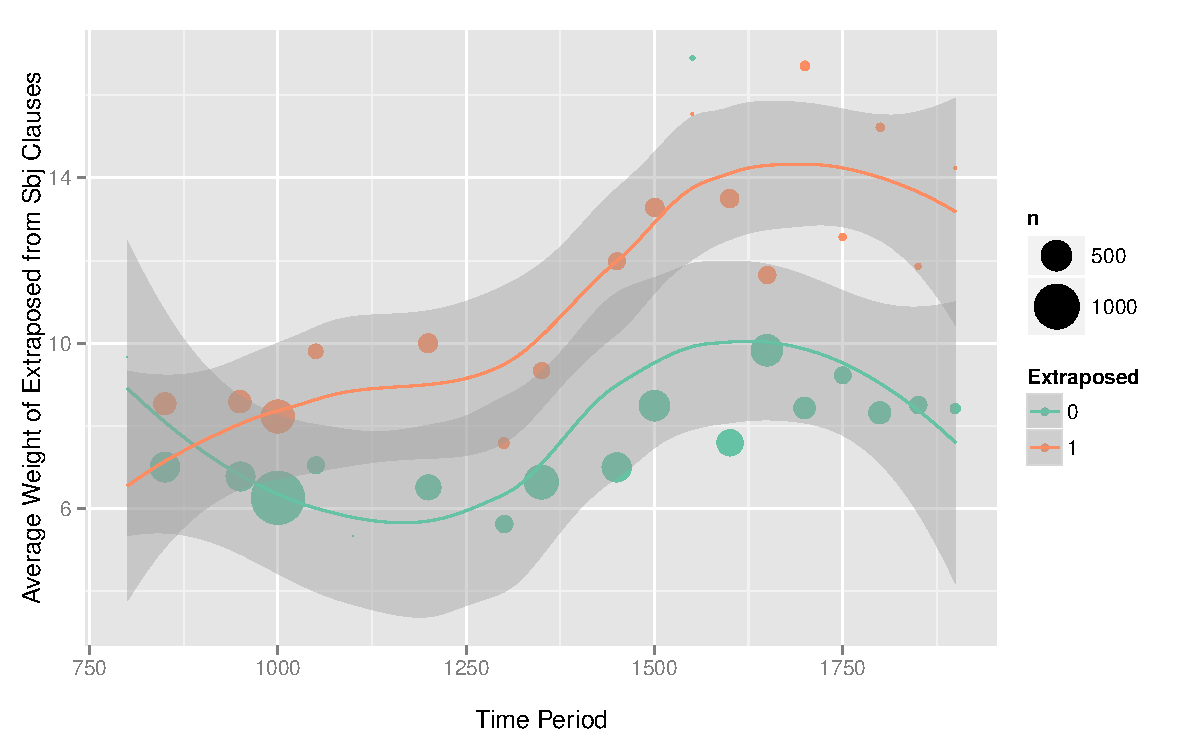
\includegraphics[width=1.1\textwidth]{exWeightYearBinned50Loessymeb.pdf}
\end{center}
\end{frame}

\begin{frame}{Icelandic, over time (N = 3486)}

\begin{center}
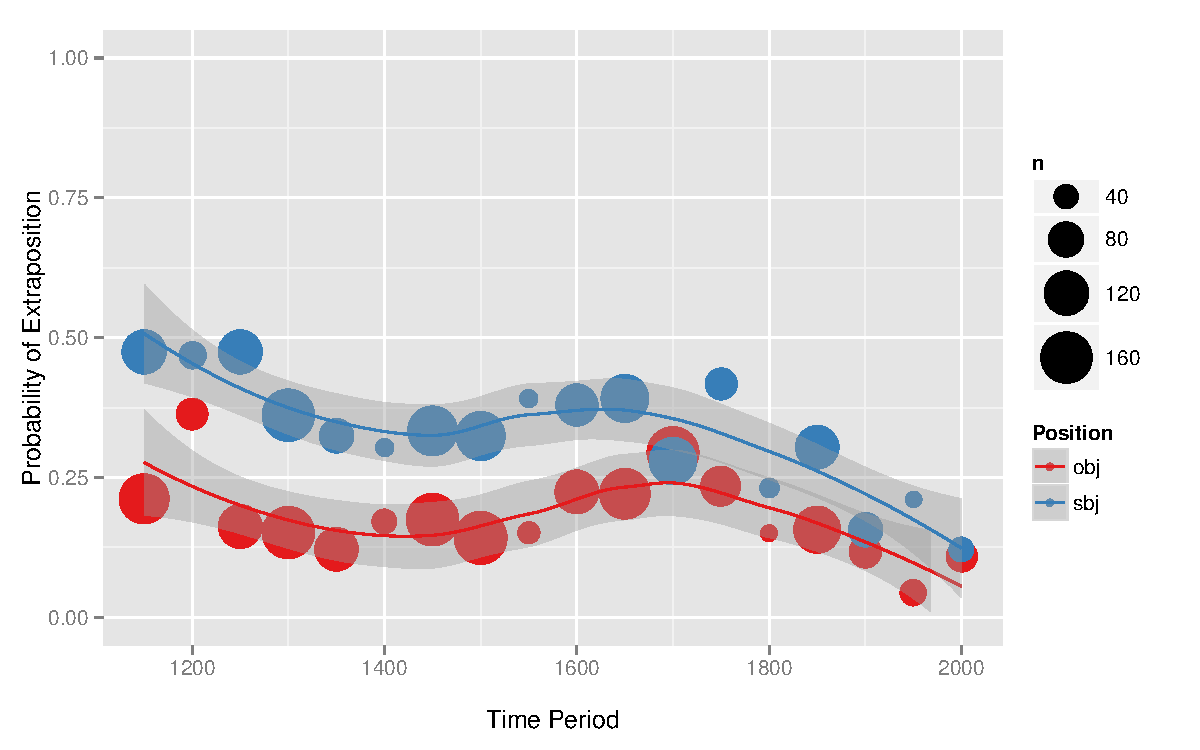
\includegraphics[width=1.1\textwidth]{exSbjObjYearBinned50Loessice.pdf}
\end{center}
\end{frame}


\begin{frame}{Icelandic, average weight over time (N = 3486)}

\begin{center}
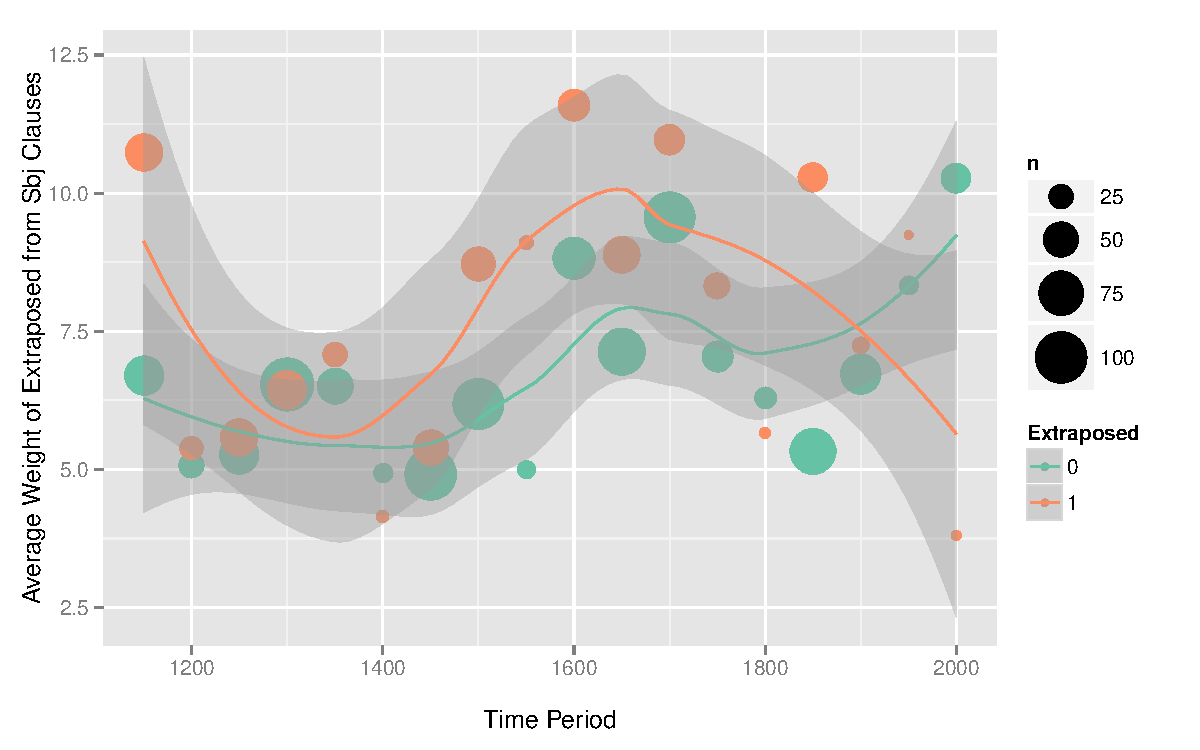
\includegraphics[width=1.1\textwidth]{exWeightYearBinned50Loessice.pdf}
\end{center}
\end{frame}



\begin{frame}{Old/Middle French, over time (N = 8207)}

\begin{center}
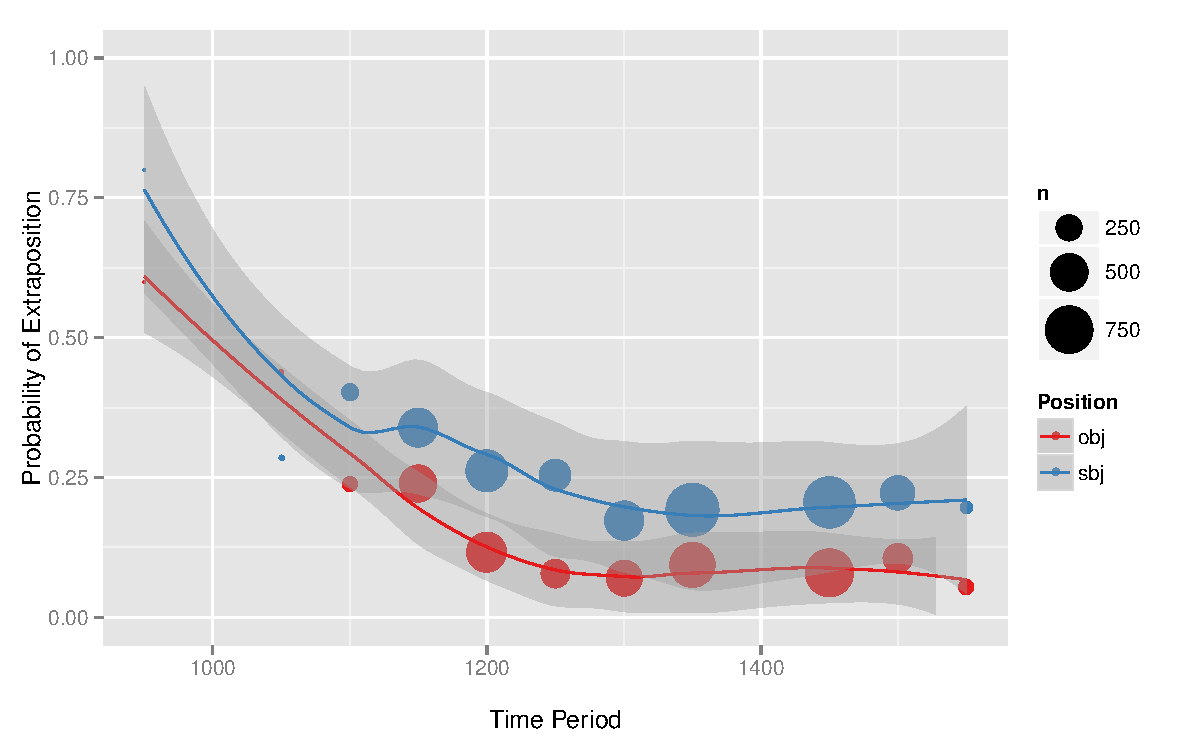
\includegraphics[width=1.1\textwidth]{exSbjObjYearBinned50Loessfre.pdf}
\end{center}
\end{frame}


\begin{frame}{French, average weight over time (N = 8207)}

\begin{center}
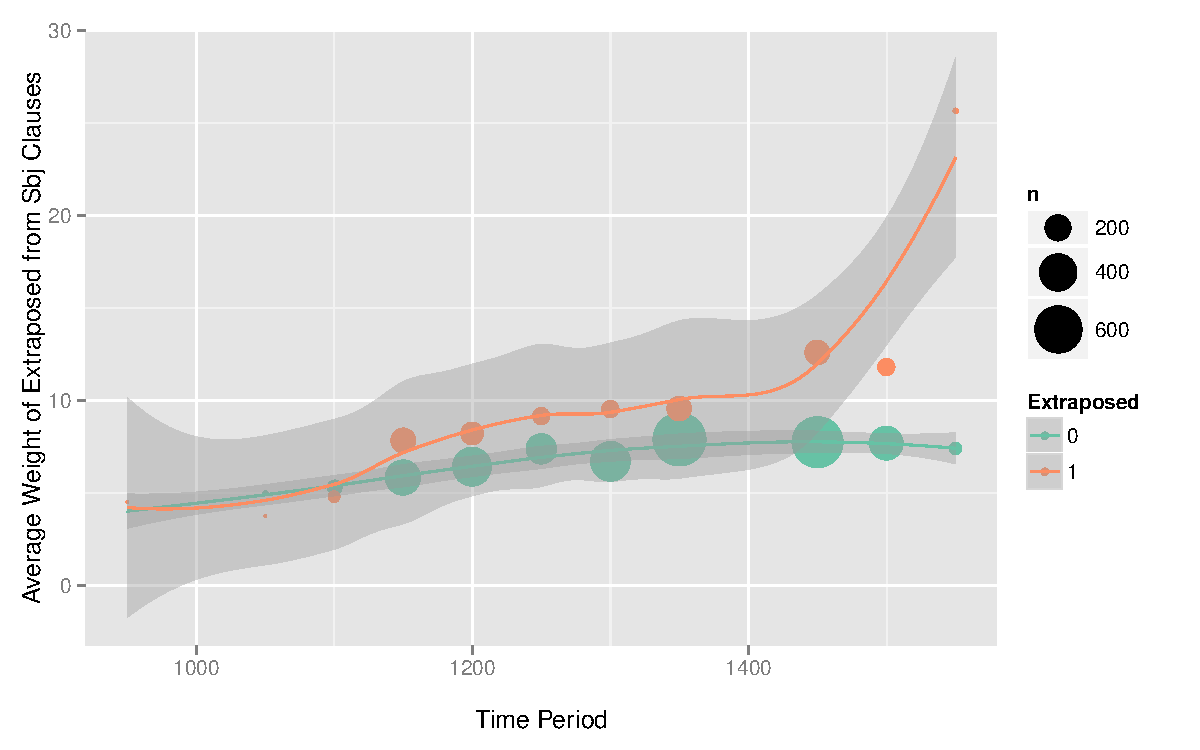
\includegraphics[width=1.1\textwidth]{exWeightYearBinned50Loessfre.pdf}
\end{center}
\end{frame}

\begin{frame}{Portuguese, over time (N = 2398)}

\begin{center}
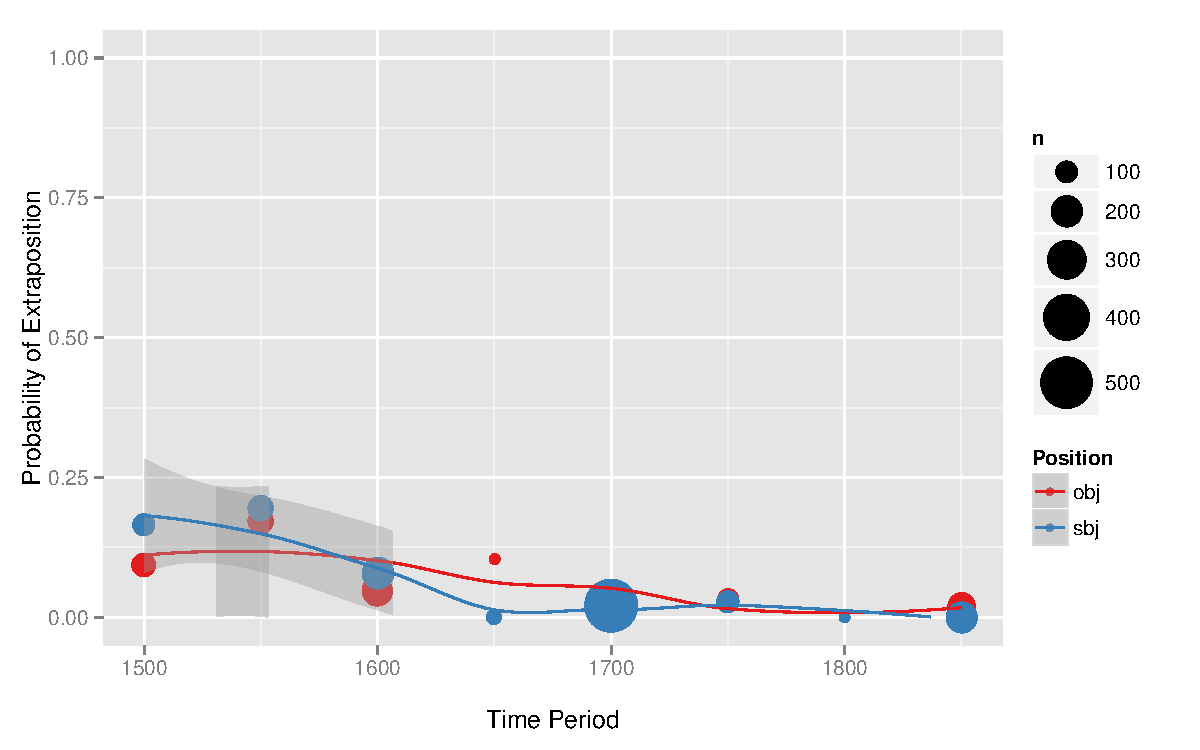
\includegraphics[width=1.1\textwidth]{exSbjObjYearBinned50Loessport.pdf}
\end{center}
\end{frame}


\begin{frame}{Portuguese, average weight over time (N = 2398)}

\begin{center}
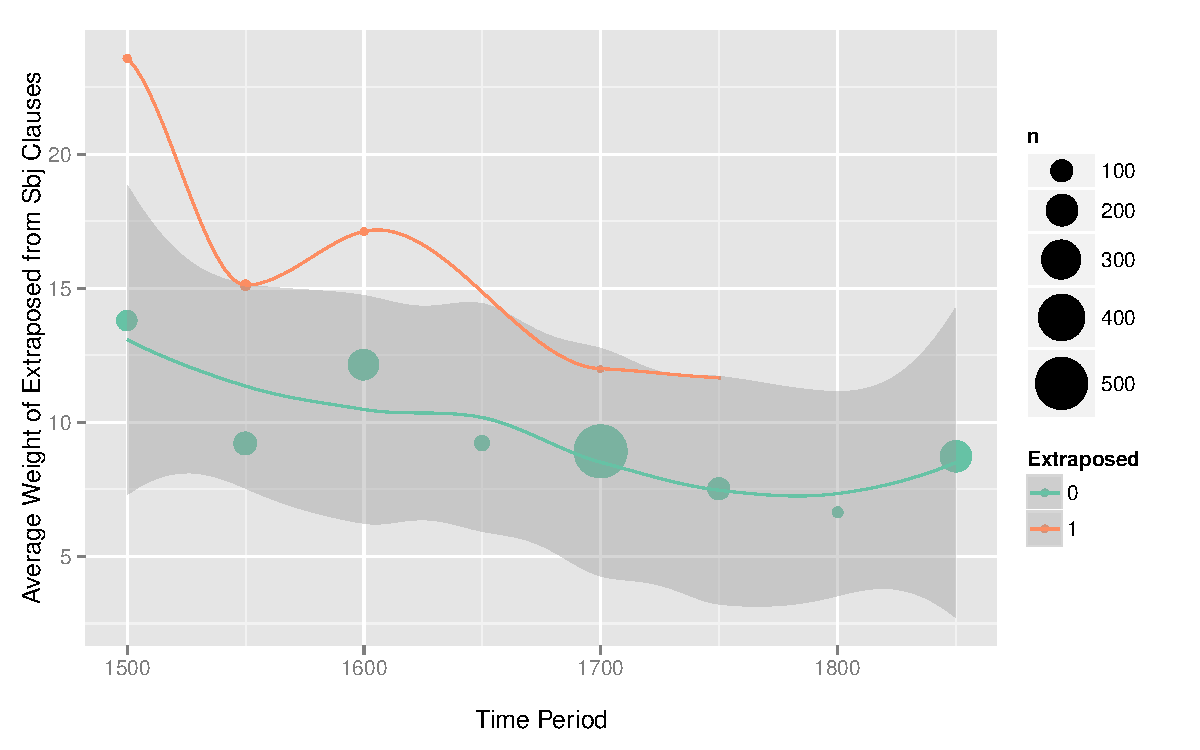
\includegraphics[width=1.1\textwidth]{exWeightYearBinned50Loessport.pdf}
\end{center}
\end{frame}



%Plots, interspersed weight and others

\begin{frame}{Change in Relative Clauses}
\begin{itemize}
	\item Why the change? \textbf{There is still some overlap in use.}
	\item Relative clause extraposition has become severely restricted in modern Portuguese \citep{cardoso2011, cardoso2012}; cause and effect?
	\item Perhaps a small selectional advantage has asserted itself in the usage-overlap, but can only do so slowly because the overlap is limited.
	\item Drift; the population (of utterances) is more likely to fixate on the majority variant over time through random death, given enough time (\citealt{moran1958}; see \citealt{nowak2006} for an overview and references).
	\item \textbf{Note:} topicalization in English has slowly declined from 1750 through the 20th c. (A. Kroch, p.c.).
\end{itemize}
\end{frame}


\section{Conclusions}





\begin{frame}{Conclusions}
	\begin{block}{Conclusions}
		\begin{itemize}
			\item Within syntax, only one formal account of optionality is available, the same one that accounts for language change: Competing Grammars (i.e. decision points in the selection of grammatical formatives).
			\item All categorical variation/optionality/change = \\Blocking Effect, Competing Grammars
			\item Blocking Effect = \\
			selection, P. of Contrast (and a domain of specialization)
			\item Thus, all categorical variation/optionality/change is reduced to interactions of Competing Grammars, selection, Principle of Contrast, and inherent mathematical properties of possible domains of specialization.
				\end{itemize}
	\end{block}
\end{frame}


\begin{frame}{Conclusions}
	\begin{block}{Conclusions}
		\begin{itemize}
			\item Competing Grammars result in replacement, specialization, or ``stable variation''.
			\item The latter is (only) the result of mapping categorical variation onto a continuous dimension of specialization.
			\item An acquisition simulation shows how stable variation can emerge under a minimal assumptions about the Principle of Contrast.
			\item Even so, the most stable variation may not be entirely stable.
			\item It is possible and desirable to extend this formal account to other domains of variation, like morphology and phonology.
		\end{itemize}
	\end{block}
	

\end{frame}

\begin{frame}{Conclusions}
	\begin{block}{Further Research}
		\begin{itemize}
			\item Now that we have questioned stability in \textbf{replacement}, we should question stability in \textbf{specialization} too.
				\begin{itemize}
					\item Perhaps both processes continue without ever stabilizing, but they bleed each other (cf. weight effect in French).
					\item The actual outcome of the change depends on the relative speeds of replacement and specialization.
					\item \textbf{Hypothesis:} the rate of specialization is fixed, given the general frequency of the construction.
				\end{itemize}
			\item The relative clause result needs to be checked, esp. for restrictive relative clauses.
			\item The topicalization change needs investigated further (ongoing research with A. Kroch).
			\item Check drift hypothesis mathematically.
				\end{itemize}
	\end{block}
\end{frame}

\begin{frame}{Conclusions}
	\begin{block}{Further Work}
		\begin{itemize}
			\item We have a hypothesis about which factors influence specialization vs replacement, as they do not \textbf{appear} to be deterministic; find a way to test it!
			\item Look into other data sets for within-speaker categorical variation specialized along a continuous dimension.
			\item Look at the set of very slow changes in more detail (where we expected stability), to control for as many factors as possible.
			\item Figure out how to appropriately parameterize phonological variation.
		\end{itemize}
	\end{block}

\end{frame}

\begin{frame}{Acknowledgements}
\begin{center}
Thank you first to Josef Fruehwald for working out many of these ideas with me, and to Anthony Kroch for much discussion of these issues. Thanks to Anton Karl Ingason for use of his CS queries. Also Aaron Ecay, Caitlin Light, Laurel Mackenzie, Ian Roberts, Meredith Tamminga, Wim van der Wurff, and participants at DiGS 15 and the LSA Institute for comments on earlier versions of this work. 
\vspace{5mm}\\
Simulation: \texttt{github.com/joelcw/tyneside/blob/master/articles/sim\_Joel.R}
\vspace{1mm}\\
Extraposition Study: \texttt{github.com/joelcw/tyneside/tree/master/extraposition}
\end{center}
\end{frame}


\begin{frame}[allowframebreaks]
\frametitle{References}
\newcommand*{\newblock}{natbib}
\bibliographystyle{linquiry2}
\bibliography{joelrefs}
\end{frame}




\end{document}